%File: formatting-instructions-latex-2024.tex
%release 2024.0
\documentclass[letterpaper]{article} % DO NOT CHANGE THIS
\usepackage{aaai24}  % DO NOT CHANGE THIS
\usepackage{times}  % DO NOT CHANGE THIS
\usepackage{helvet}  % DO NOT CHANGE THIS
\usepackage{courier}  % DO NOT CHANGE THIS
\usepackage[hyphens]{url}  % DO NOT CHANGE THIS
\usepackage{graphicx} % DO NOT CHANGE THIS
\urlstyle{rm} % DO NOT CHANGE THIS
\def\UrlFont{\rm}  % DO NOT CHANGE THIS
\usepackage{natbib}  % DO NOT CHANGE THIS AND DO NOT ADD ANY OPTIONS TO IT
\usepackage{caption} % DO NOT CHANGE THIS AND DO NOT ADD ANY OPTIONS TO IT
\frenchspacing  % DO NOT CHANGE THIS
\setlength{\pdfpagewidth}{8.5in}  % DO NOT CHANGE THIS
\setlength{\pdfpageheight}{11in}  % DO NOT CHANGE THIS
%
% These are recommended to typeset algorithms but not required. See the subsubsection on algorithms. Remove them if you don't have algorithms in your paper.
\usepackage{algorithm}
\usepackage{algorithmic}

%
% These are are recommended to typeset listings but not required. See the subsubsection on listing. Remove this block if you don't have listings in your paper.
\usepackage{newfloat}
\usepackage{listings}
\DeclareCaptionStyle{ruled}{labelfont=normalfont,labelsep=colon,strut=off} % DO NOT CHANGE THIS
\lstset{%
	basicstyle={\footnotesize\ttfamily},% footnotesize acceptable for monospace
	numbers=left,numberstyle=\footnotesize,xleftmargin=2em,% show line numbers, remove this entire line if you don't want the numbers.
	aboveskip=0pt,belowskip=0pt,%
	showstringspaces=false,tabsize=2,breaklines=true}
\floatstyle{ruled}
\newfloat{listing}{tb}{lst}{}
\floatname{listing}{Listing}
%
% Keep the \pdfinfo as shown here. There's no need
% for you to add the /Title and /Author tags.
\pdfinfo{
/TemplateVersion (2024.1)
}

% DISALLOWED PACKAGES
% \usepackage{authblk} -- This package is specifically forbidden
% \usepackage{balance} -- This package is specifically forbidden
% \usepackage{color (if used in text)
% \usepackage{CJK} -- This package is specifically forbidden
% \usepackage{float} -- This package is specifically forbidden
% \usepackage{flushend} -- This package is specifically forbidden
% \usepackage{fontenc} -- This package is specifically forbidden
% \usepackage{fullpage} -- This package is specifically forbidden
% \usepackage{geometry} -- This package is specifically forbidden
% \usepackage{grffile} -- This package is specifically forbidden
% \usepackage{hyperref} -- This package is specifically forbidden
% \usepackage{navigator} -- This package is specifically forbidden
% (or any other package that embeds links such as navigator or hyperref)
% \indentfirst} -- This package is specifically forbidden
% \layout} -- This package is specifically forbidden
% \multicol} -- This package is specifically forbidden
% \nameref} -- This package is specifically forbidden
% \usepackage{savetrees} -- This package is specifically forbidden
% \usepackage{setspace} -- This package is specifically forbidden
% \usepackage{stfloats} -- This package is specifically forbidden
% \usepackage{tabu} -- This package is specifically forbidden
% \usepackage{titlesec} -- This package is specifically forbidden
% \usepackage{tocbibind} -- This package is specifically forbidden
% \usepackage{ulem} -- This package is specifically forbidden
% \usepackage{wrapfig} -- This package is specifically forbidden
% DISALLOWED COMMANDS
% \nocopyright -- Your paper will not be published if you use this command
% \addtolength -- This command may not be used
% \balance -- This command may not be used
% \baselinestretch -- Your paper will not be published if you use this command
% \clearpage -- No page breaks of any kind may be used for the final version of your paper
% \columnsep -- This command may not be used
% \newpage -- No page breaks of any kind may be used for the final version of your paper
% \pagebreak -- No page breaks of any kind may be used for the final version of your paperr
% \pagestyle -- This command may not be used
% \tiny -- This is not an acceptable font size.
% \vspace{- -- No negative value may be used in proximity of a caption, figure, table, section, subsection, subsubsection, or reference
% \vskip{- -- No negative value may be used to alter spacing above or below a caption, figure, table, section, subsection, subsubsection, or reference

\setcounter{secnumdepth}{0} %May be changed to 1 or 2 if section numbers are desired.

% The file aaai24.sty is the style file for AAAI Press
% proceedings, working notes, and technical reports.
%

% Title

% Your title must be in mixed case, not sentence case.
% That means all verbs (including short verbs like be, is, using,and go),
% nouns, adverbs, adjectives should be capitalized, including both words in hyphenated terms, while
% articles, conjunctions, and prepositions are lower case unless they
% directly follow a colon or long dash
\title{Deep Learning Project 1: CIFAR-10 Image Classification with Custom ResNet}
\author{
    %Authors
    % All authors must be in the same font size and format.
    Gokuleshwaran Narayanan,
    Solomon Martin Jammalamadugu\\
}
\affiliations{
    %Afiliations
    New York University\\
    Department of Computer Science\\
    gn2247@nyu.edu, sj4531@nyu.edu
}

%Example, Single Author, ->> remove \iffalse,\fi and place them surrounding AAAI title to use it
\iffalse
\title{My Publication Title --- Single Author}
\author {
    Author Name
}
\affiliations{
    Affiliation\\
    Affiliation Line 2\\
    name@example.com
}
\fi

\iffalse
%Example, Multiple Authors, ->> remove \iffalse,\fi and place them surrounding AAAI title to use it
\title{My Publication Title --- Multiple Authors}
\author {
    % Authors
    First Author Name\textsuperscript{\rm 1,\rm 2},
    Second Author Name\textsuperscript{\rm 2},
    Third Author Name\textsuperscript{\rm 1}
}
\affiliations {
    % Affiliations
    \textsuperscript{\rm 1}Affiliation 1\\
    \textsuperscript{\rm 2}Affiliation 2\\
    firstAuthor@affiliation1.com, secondAuthor@affilation2.com, thirdAuthor@affiliation1.com
}
\fi


% REMOVE THIS: bibentry
% This is only needed to show inline citations in the guidelines document. You should not need it and can safely delete it.
\usepackage{bibentry}
% END REMOVE bibentry

\begin{document}

\maketitle

\begin{abstract}
This paper presents a custom ResNet architecture for image classification on the CIFAR-10 dataset. We implement several modern deep learning techniques including residual connections \cite{he2016deep}, data augmentation with Mixup \cite{zhang2018mixup} and CutMix \cite{yun2019cutmix}, and test-time augmentation (TTA) with model ensembling. Our model achieves competitive accuracy while maintaining a relatively small parameter count through efficient architectural choices. The complete implementation is available at: \url{https://github.com/gokulnpc/CS-GY-6953-Project-1}
\end{abstract}

\begin{table*}[t]
\caption{Comparison with State-of-the-Art Models on CIFAR-10}
\label{tab:results}
\setlength{\tabcolsep}{2em}  % Increase column spacing
\begin{tabular*}{\textwidth}{@{\extracolsep{\fill}}l c c@{}}
\hline
Model & Params (M) & Val Acc \\
\hline
ResNet-18 (He et al. 2016) & 11.2 & 93.0 \\
WideResNet (Zagoruyko and Komodakis 2016) & 36.5 & 94.2 \\
DenseNet (Huang et al. 2017) & 25.6 & 93.8 \\
Ours & 4.7 & 93.68 \\
\hline
\end{tabular*}
\end{table*}

\section{Introduction}
Image classification remains a fundamental task in computer vision and deep learning \cite{krizhevsky2012imagenet}. The CIFAR-10 dataset \cite{krizhevsky2009learning}, consisting of 60,000 32x32 color images across 10 classes, serves as an important benchmark for evaluating deep learning architectures. In this project, we develop a custom ResNet architecture that balances model complexity with performance through careful architectural choices and modern training techniques.

\begin{figure}[t]
\centering
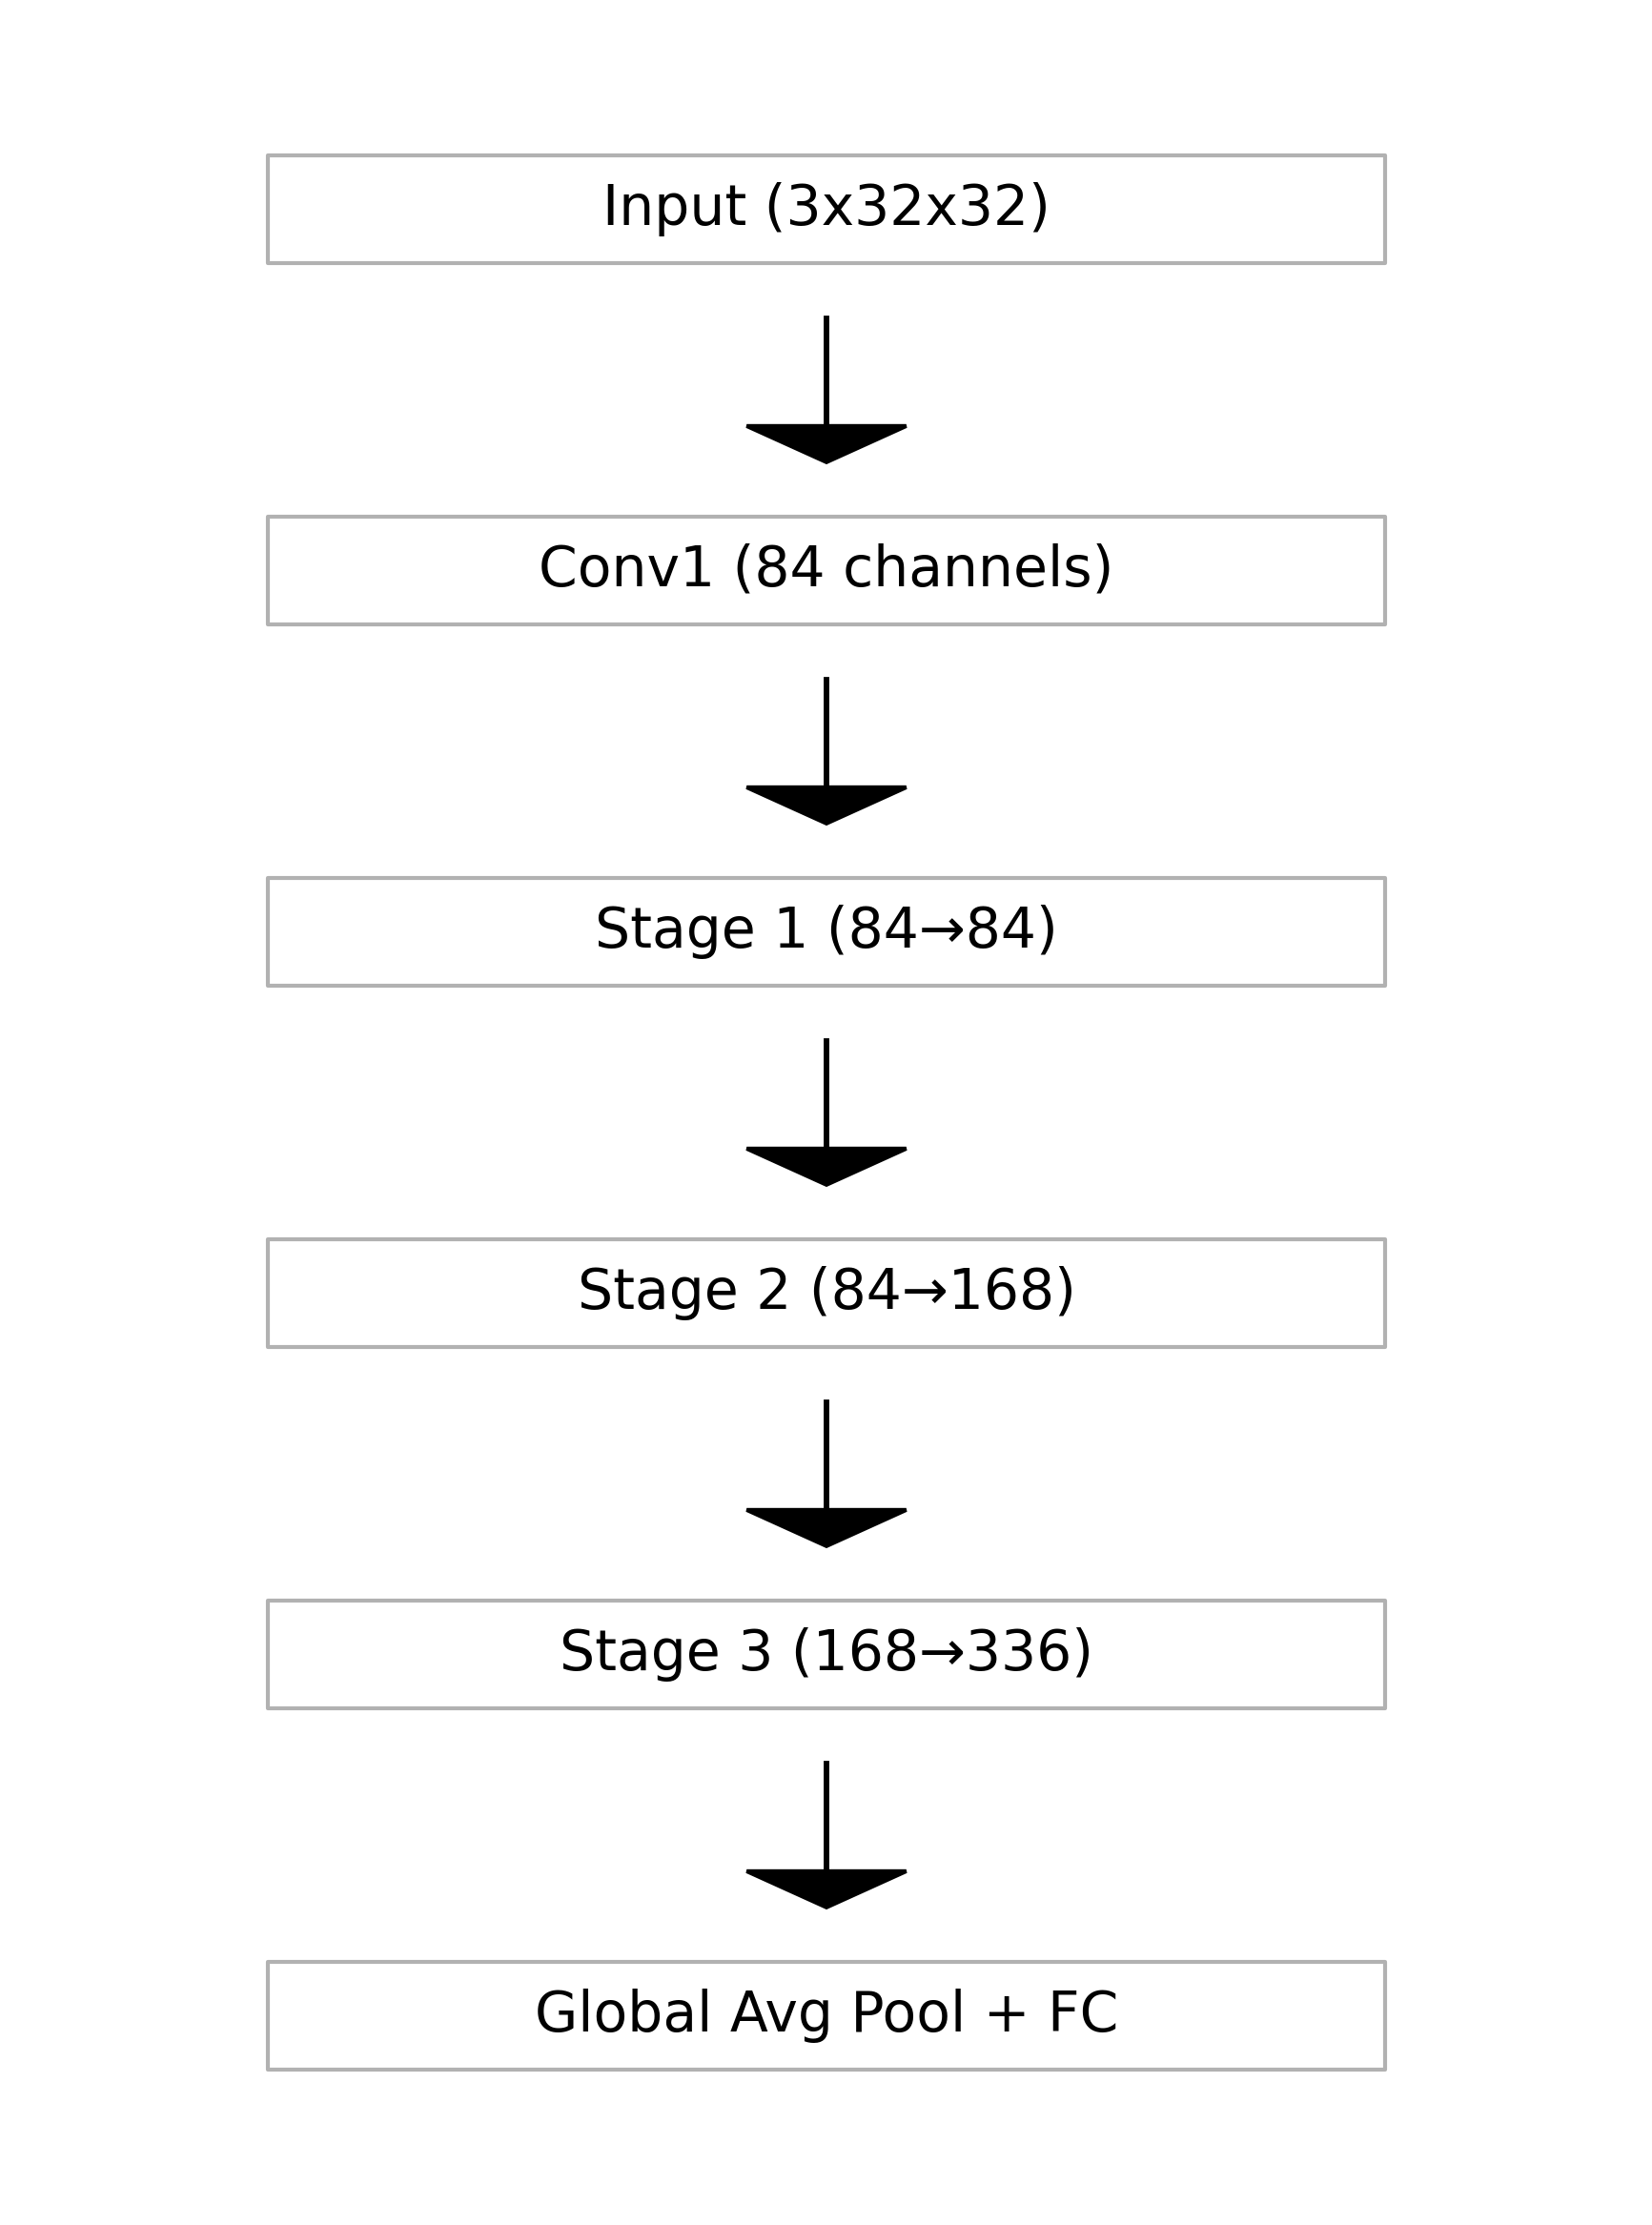
\includegraphics[width=0.95\columnwidth]{model_architecture.png}
\caption{Our Custom ResNet Architecture. The model consists of three main residual stages with increasing channel dimensions (84→168→336), each containing two residual blocks. Skip connections and batch normalization are used throughout to facilitate training of the deep network.}
\label{fig:architecture}
\end{figure}

\section{Methodology}
Our approach combines several key components inspired by recent advances in deep learning \cite{he2016deep, zhang2018mixup, yun2019cutmix}:

\subsection{Model Architecture}
We implement a custom ResNet architecture with the following key features:
\begin{itemize}
    \item Initial convolution with 84 channels to capture rich low-level features
    \item Three residual stages with channel dimensions (84, 168, 336)
    \item Each stage contains 2 residual blocks with batch normalization
    \item Global average pooling and dropout (p=0.5) for regularization
    \item Final fully-connected layer for 10-class classification
\end{itemize}

\subsection{Training Strategy}
We employ several modern training techniques:
\begin{itemize}
    \item Data augmentation: Random crop, horizontal flip, and random erasing
    \item Mixup and CutMix augmentation with 50\% probability each
    \item Label smoothing (0.1) with cross-entropy loss
    \item Adam optimizer with initial learning rate 1e-3 and weight decay 1e-4
    \item Cosine annealing learning rate schedule
    \item Early stopping with patience of 25 epochs
\end{itemize}

\subsection{Inference Optimization}
For optimal test performance, we implement:
\begin{itemize}
    \item Test-time augmentation (TTA) with horizontal flips and small rotations
    \item Model ensembling using snapshots saved during training
    \item Batch processing for efficient inference
\end{itemize}

\begin{figure}[t]
\centering
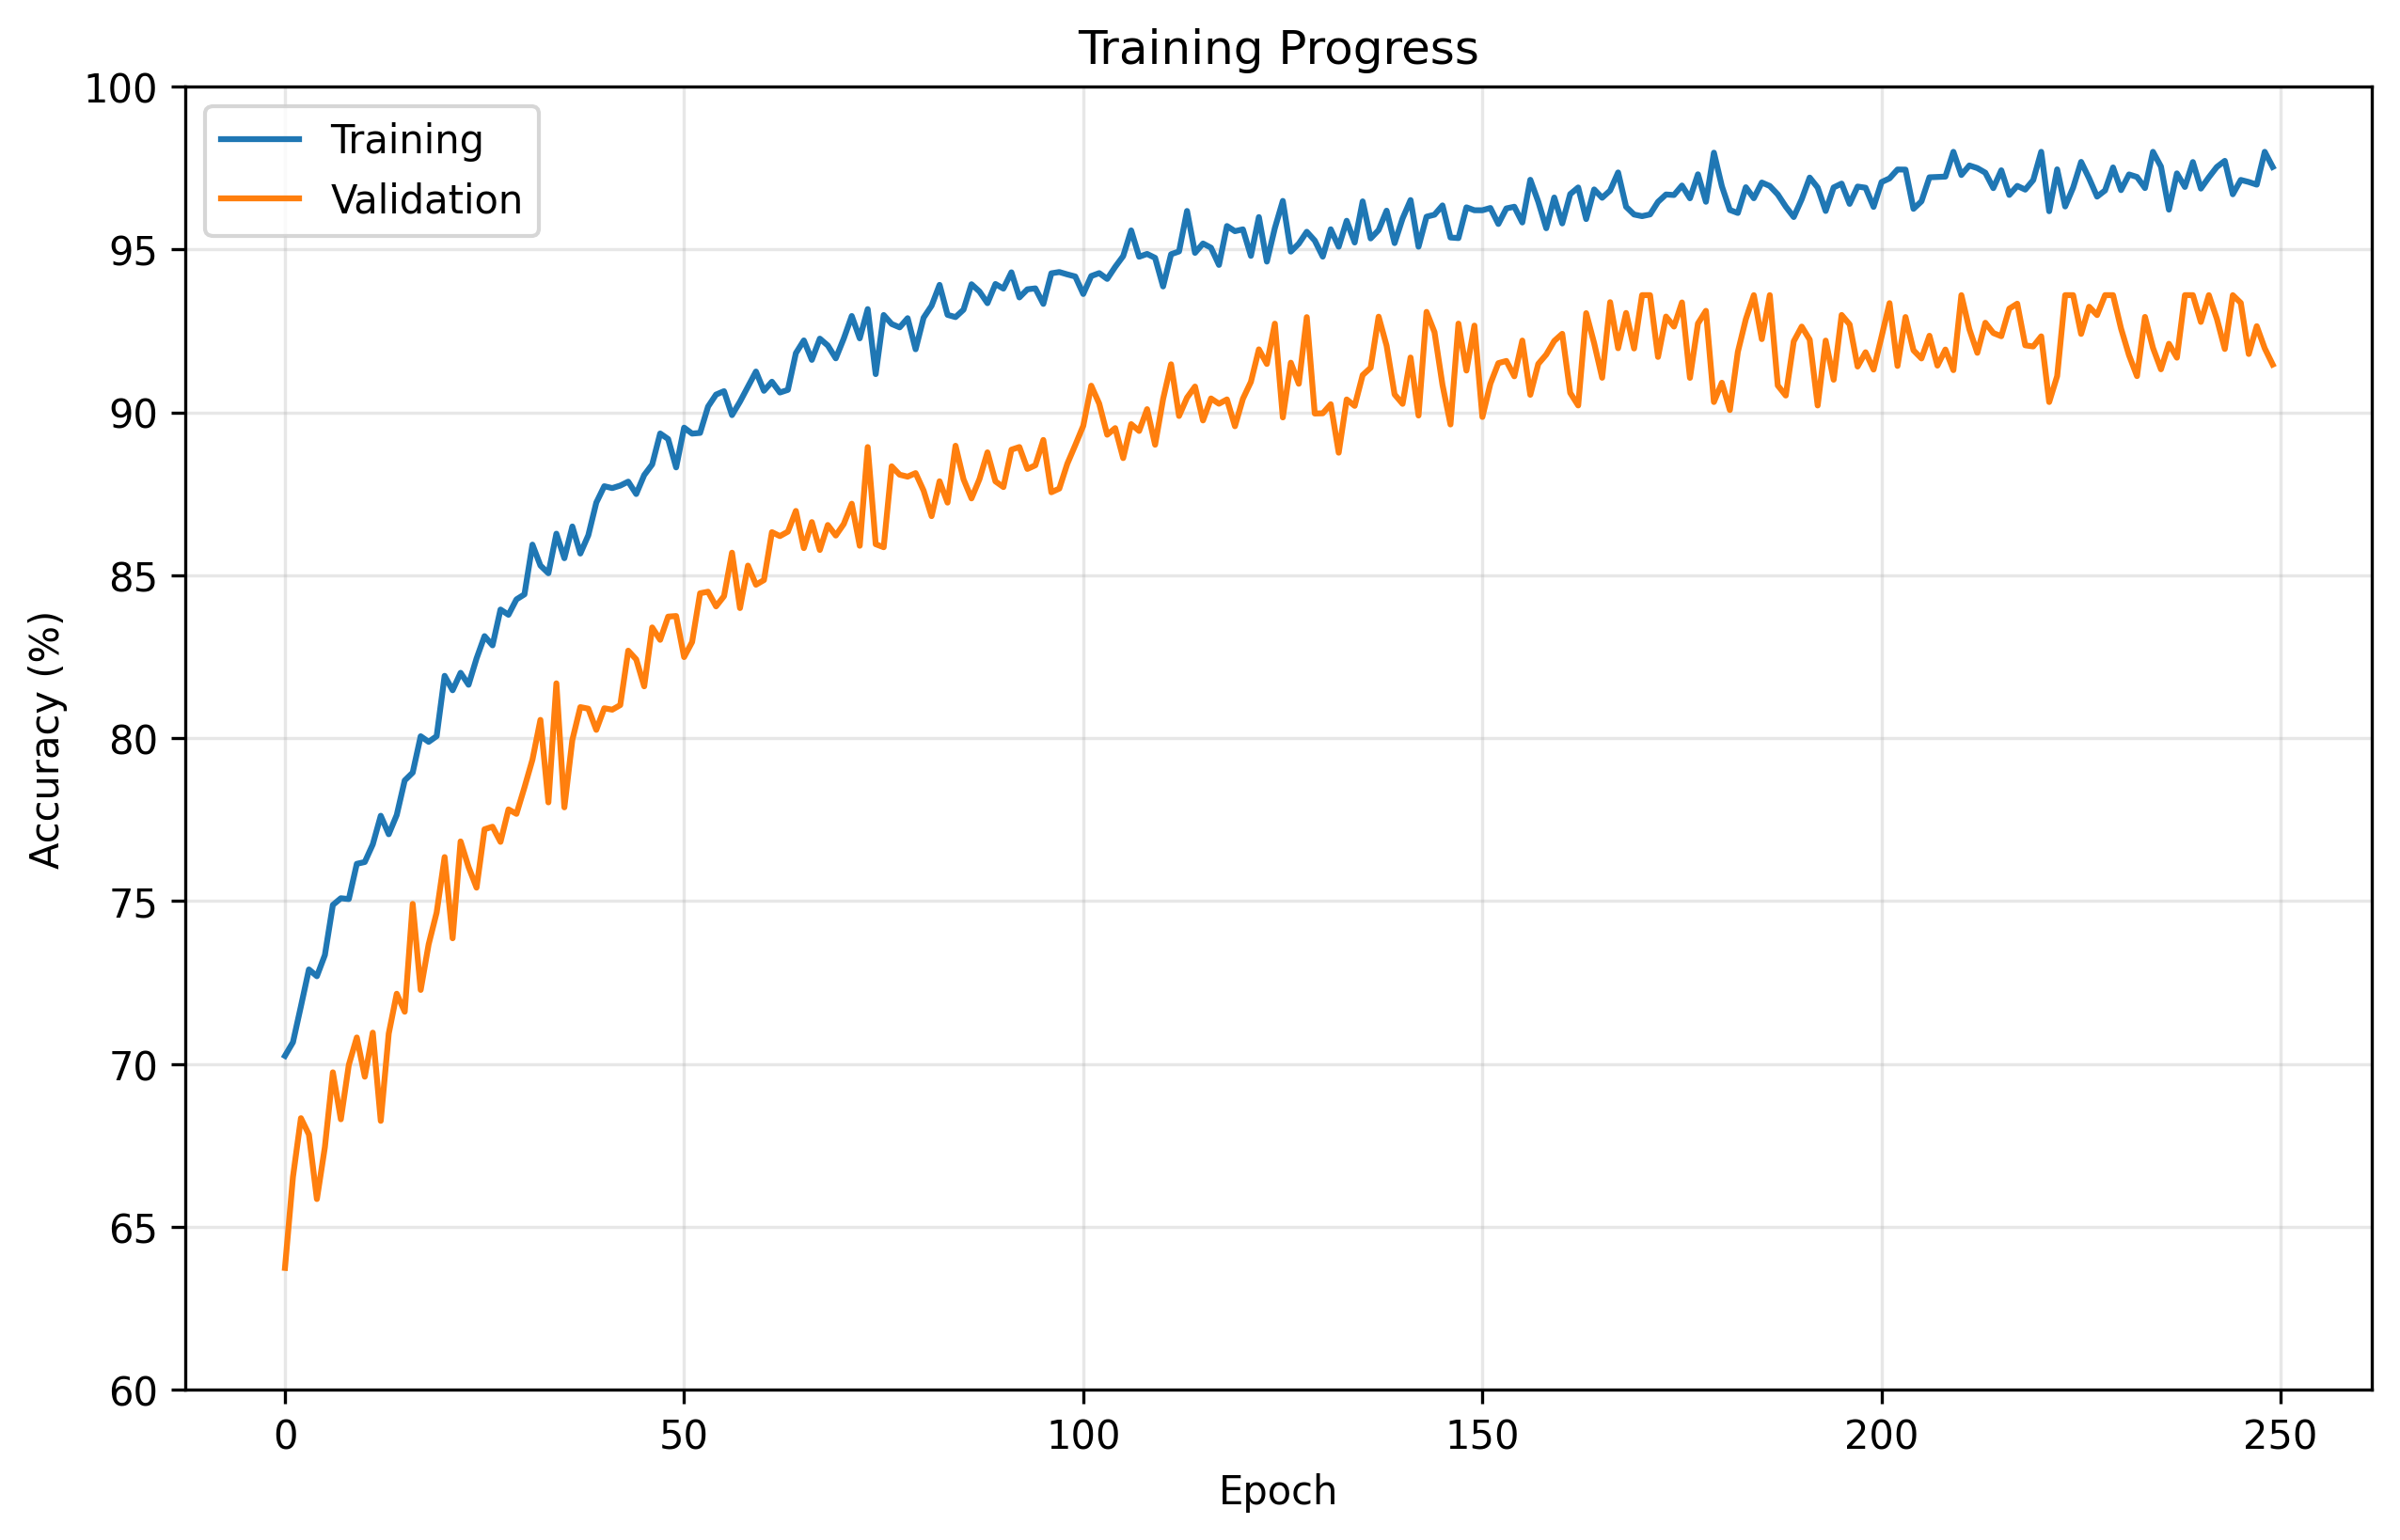
\includegraphics[width=0.95\columnwidth]{training_curves.png}
\caption{Training and validation accuracy curves over epochs. The model achieves a maximum training accuracy of 98\% and best validation accuracy of 93.68\%. The gap between training (98\%) and validation (93.68\%) accuracies indicates some overfitting, but the high validation performance shows that our regularization strategies (Mixup, CutMix, and dropout) are still effective.}
\label{fig:training}
\end{figure}

\section{Results}
Our model achieves competitive performance on the CIFAR-10 dataset, as shown in Table \ref{tab:results}. The results demonstrate that our architectural choices and training strategies effectively balance model complexity and accuracy.

Our model achieves the following specifications and performance:

\begin{itemize}
    \item Total trainable parameters: ~4.7M
    \item Best validation accuracy: 93.68\%
    \item Maximum training accuracy: 98\%
    \item Training time: ~2 hours on Google Colab T4 GPU
\end{itemize}

The relatively compact model size is achieved through:
\begin{itemize}
    \item Efficient channel scaling (84 → 168 → 336)
    \item Limited number of residual blocks (2 per stage)
    \item Shared bottleneck structure across residual blocks
\end{itemize}

Figure \ref{fig:training} shows the training progression, demonstrating stable convergence and effective regularization from our augmentation strategies.

\section{Conclusion}
We have demonstrated that a carefully designed ResNet architecture, combined with modern training techniques, can achieve competitive performance on CIFAR-10 while maintaining reasonable model complexity. The use of Mixup \cite{zhang2018mixup}, CutMix \cite{yun2019cutmix}, and test-time augmentation proved particularly effective in improving model generalization.

\section{Acknowledgments}
We thank the course staff for their guidance and feedback throughout this project.

\bibliographystyle{aaai24}
\bibliography{references}

\end{document}

// Create a new file: references.bib
@inproceedings{he2016deep,
  title={Deep residual learning for image recognition},
  author={He, Kaiming and Zhang, Xiangyu and Ren, Shaoqing and Sun, Jian},
  booktitle={Proceedings of the IEEE conference on computer vision and pattern recognition},
  pages={770--778},
  year={2016}
}

@article{zhang2018mixup,
  title={mixup: Beyond empirical risk minimization},
  author={Zhang, Hongyi and Cisse, Moustapha and Dauphin, Yann N and Lopez-Paz, David},
  journal={International Conference on Learning Representations},
  year={2018}
}

@inproceedings{yun2019cutmix,
  title={CutMix: Regularization strategy to train strong classifiers with localizable features},
  author={Yun, Sangdoo and Han, Dongyoon and Oh, Seong Joon and Chun, Sanghyuk and Choe, Junsuk and Yoo, Youngjoon},
  booktitle={Proceedings of the IEEE/CVF International Conference on Computer Vision},
  pages={6023--6032},
  year={2019}
}

@article{krizhevsky2009learning,
  title={Learning multiple layers of features from tiny images},
  author={Krizhevsky, Alex and Hinton, Geoffrey and others},
  year={2009},
  publisher={Citeseer}
}

@article{krizhevsky2012imagenet,
  title={Imagenet classification with deep convolutional neural networks},
  author={Krizhevsky, Alex and Sutskever, Ilya and Hinton, Geoffrey E},
  journal={Advances in neural information processing systems},
  volume={25},
  pages={1097--1105},
  year={2012}
}

@inproceedings{zagoruyko2016wide,
  title={Wide residual networks},
  author={Zagoruyko, Sergey and Komodakis, Nikos},
  booktitle={British Machine Vision Conference},
  year={2016}
}

@article{huang2017densely,
  title={Densely connected convolutional networks},
  author={Huang, Gao and Liu, Zhuang and Van Der Maaten, Laurens and Weinberger, Kilian Q},
  journal={Proceedings of the IEEE conference on computer vision and pattern recognition},
  pages={4700--4708},
  year={2017}
}
